\section{Methodology}\label{sec:review}

The application architecture was designed using the Model-view-controller approach (MVC, "model-view-controller"). It is a software design pattern for implementing user interfaces on computers. It divides a given software application into three interconnected parts, so as to separate internal representations of information from the ways that information is presented to or accepted from the user. This design pattern is often used for creation of an architectural frame when you pass from the theory to implementation in the specific data domain.

The main application objective of this concept is the separation of business logic (model) from its visualization (view). Due to such division the possibility of reuse raises. 
As with other software architectures, MVC expresses the "core of the solution" to a problem while allowing it to be adapted for each system.

The central component of MVC, the model, captures the behavior of the application in terms of its problem domain, independent of the user interface.

\begin {itemize}
\item The model directly manages the data, logic, and rules of the application.
\item A view can be any output representation of information, such as a chart or a diagram. Multiple views of the same information are possible, such as a bar chart for management and a tabular view for accountants.
\item The third part, the controller, accepts input and converts it to commands for the model or view.
\end {itemize}

In addition to dividing the application into three kinds of components, the model-view-controller design defines the interactions between them.

\begin {itemize}
\item A model stores data that is retrieved according to commands from the controller and displayed in the view.
\item A view generates new output to the user based on changes in the model.
\item A controller can send commands to the model to update the model's state (e.g., editing a document). It can also send commands to its associated view to change the view's presentation of the model (e.g., by scrolling through a document).
\end {itemize}

In the implementation of the required web service each request is intercepted by the global Front-controller which determines by specific parameters (URI) to what controller to transfer the received request. The controller processes the request and creates model. The Front-controller fills the view with the model data and returns the received result to the browser. The diagram of the request processing in Spring on the picture \ref{fig:requestProcessing} is given below.



\begin{figure}[tbh]
\centering
\caption{The diagram of the request processing in Spring}
\label{fig:requestProcessing}
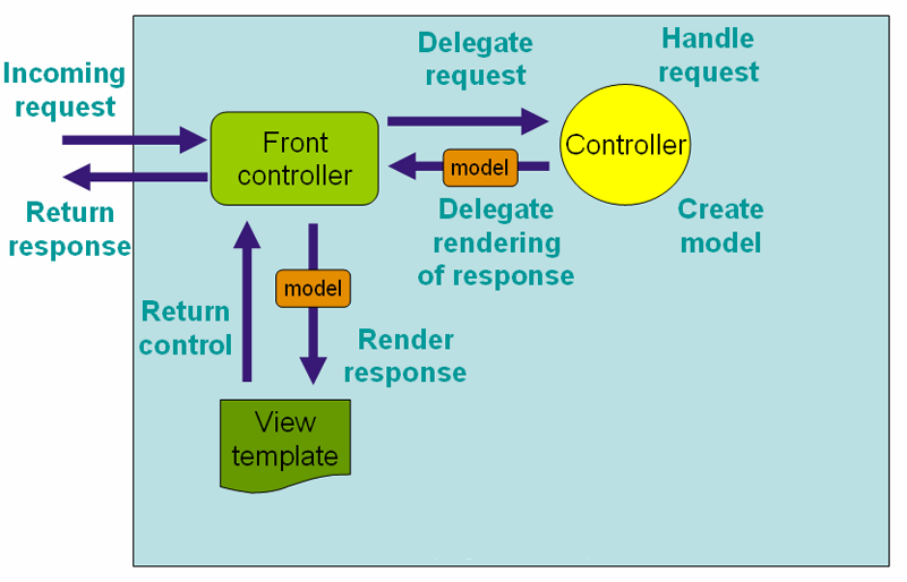
\includegraphics[width=\linewidth]{requestProcessing}
\end{figure}


The web service was implemented using the classical algorithm called Word Count. The task is formulated as follows: there is a large number of tweets. We check each tweet for the existence of the specific keyword: we look for an index i of the first entrance of substring in a tweet line - if an index non-negative, then we increment the counter. Further we look for an index of the following keyword appearance since the i+1 item, incrementing the counter in case of success. After analyzing all the tweet, the number of keyword detection in it is added with its quantity in the previous already viewed tweets.  
Twitter has a restriction of requests amount because of probability of the excessive load on their servers. Therefore the solution with data cached in the memory was developed.
